%++++++++++++++++++++++++++++++++++++++++
% Don't modify this section unless you know what you're doing!
\documentclass[letterpaper,11pt]{article}
\linespread{1.0}
% \usepackage{natbib}
\bibliographystyle{unsrtnat}
\usepackage{tabularx} % extra features for tabular environment
\usepackage{amsmath}  % improve math presentation
\usepackage{graphicx} % takes care of graphic including machinery
\usepackage[margin=1in,letterpaper]{geometry} % decreases margins
\usepackage{cite} % takes care of citations
\usepackage[final]{hyperref} % adds hyper links inside the generated pdf file
\usepackage[boxed]{algorithm}
\usepackage[noend]{algpseudocode}
\algrenewcommand{\algorithmiccomment}[1]{\hskip 1em \texttt{// #1}}
\hypersetup{
	colorlinks=true,       % false: boxed links; true: colored links
	linkcolor=blue,        % color of internal links
	citecolor=blue,        % color of links to bibliography
	filecolor=magenta,     % color of file links
	urlcolor=blue         
}
%+++++++++++++++++++++++++++++++++++++++
\begin{document}

\title{EECS 498: Introduction to Algorithmic Robotics \\\textbf{Localization: Kalman Filter and Particle Filter}}
\author{Hanxi Wan, Che Chen}
\date{\today}
\maketitle

\section{Introduction}

In localization problems, we want to know the current state (position, orientation, etc.) of objects as precisely as possible. However, due to the errors in measurements, data from sensors need to be processed to generate closer estimate of the state. Kalman filter and particle filter are two methods applied in this project to track the state of objects. Given indirect measurable variables (data from sensors), these two methods can give an estimate on the state which can not be directly measured (actual position, etc.).

The localization problems are widely seen and thus are of great significance. Robots need to be informed of its pose in the environment to carry out tasks. When driving, the navigators need to know the precise location of our vehicles. Filters can be applied to data from GPS and gyroscopes to reduce error.

The objective of this project is to compare the performances of Kalman filter and particle filter in the same scenario. A PR2 robot is executed to go through a path in an environment with obstacles and a location sensor is simulated to give the position of the robot with random error. Kalman filter and particle filter are applied respectively to give the estimate of pose of the robot. Their accuracy will be compared.


\section{Theory}

Kalman filter takes in a prior Gaussian probability distribution of the previous state and sensor measurements to compute a probability distribution of the current state. It firstly predicts the current state by applying dynamics on the previous state. Then, it corrects the prediction using sensor measurement. This prediction-correction cycle tracks the state continuously when the object is moving. \cite{kf}

The key feature of Kalman filter is that it represents state and measurement with Gaussians to deal with continuous models. However, not all errors are from Gaussian distribution. To deal with errors from arbitrary probability distribution, particle filter can be used.

Particle filter samples from implicit distribution of the state and associates each sample (called particle) with its weight. The weight of particle represents how likely it is to be the true state. At each iteration the weight of state applied with dynamics is updated according to the sensor data, and the particles are re-sampled based on the updated weight. \cite{particle} The most likely state can be extracted from the weighted particles. The accuracy generally increase as the number of iterations goes up.




\section{Implementation}

\subsection{Environment and Robot Path}
A plane scenario which contains walls looked like the word "EECS" is built for the PR2 robot to move through. The irregularly shaped walls simulate the obstacles that robots may meet with in reality. 

The robot's path between walls is pre-deterimined. This is a project on the performances of filters on prediction of state, so path planning is not the focus and thus is given to the robot. The path starts from the left bottom of the walls, walks between the walls and ends at the right bottom of the walls, shown as red dots in Figure \ref{fig:path}

\begin{figure}[ht] 
	\centering
	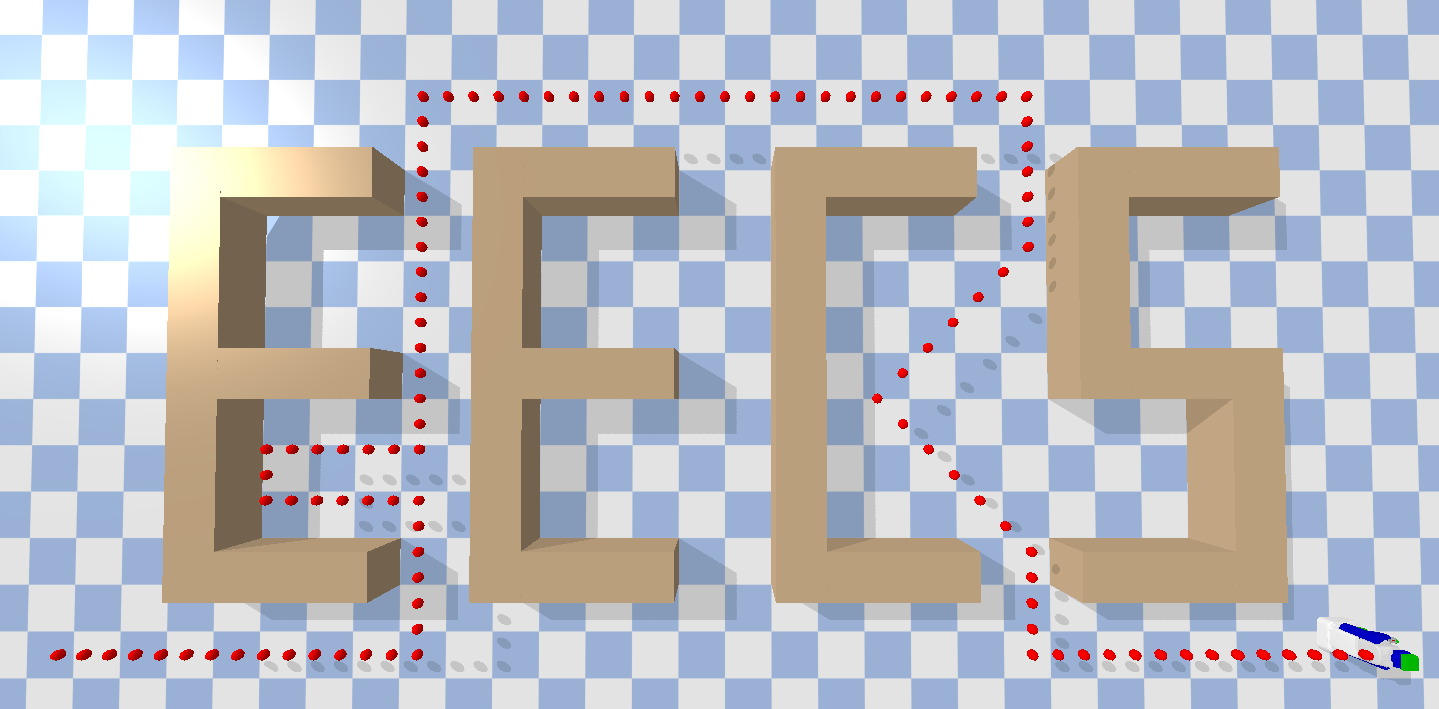
\includegraphics[width=0.5\textwidth]{path.png}
	\caption{Pre-determined Path Between the Walls.}
	\label{fig:path}
\end{figure}

The path is stored as a sequence of poses with a modifiable step length, where each pose represents a different state. The breakdown of path into sequence of poses makes it easier for the robot to execute. The state is described by the position on x-axis and y-axis, as well as the angle $\theta$ from the x-axis:
$$x_t = [x\; y\; \theta]^T$$

\subsection{Location Sensor}
The measurement from sensor is generated by adding noise to the actual pose. There are totally two scenarios in our Implementation of sensor:

\begin{enumerate}
	\item The noise is extracted from Gaussian probability distribution. This scenario meets the requirement of Kalman filter. The covariance matrix of the distribution $\Sigma_{sensor}$ is tuned according to the size of the map. In this scenario, $\delta_t$ is sampled from $\Delta \sim \mathcal{N}(0,\,\Sigma_{sensor})\,$
	\item The noise is extracted from a Uniform probability distribution near the actual pose. The boundary of the distribution $b_{sensor}$ is tuned according to the size of the map. In this scenario, $\delta_t$ is sampled from $\Delta \sim \mathbf{U}(-b_{sensor},\,b_{sensor})\,$.
\end{enumerate}

The sensor measurement is given by
	$$z_t = C_t x_t + \delta_t,$$
	where $C_t = \begin{bmatrix}
		1 & 0 & 0\\
		0 & 1 & 0\\
		0 & 0 & 1
	   \end{bmatrix}$is a matrix that maps state $x_t$ to measurement $z_t$.

\subsection{Robot Action}
The action vector of robot should be the difference between target state and current state. In the implementation, the target state $x_{p,t+1}$ is given by the path, and the current state is replaced by the estimated state $x_{e,t-1}$ since the actual state is unknown to the robot.

To simulate the control error which occurs in the real world, we add actuation noise $\varepsilon_t$ to the action vector. The noise is sampled from $\epsilon \sim \mathcal{N}(0,\,\Sigma_{action})\,$, where covariance matrix $\Sigma_{action}$ is tuned according to the size of the map.

After all, the action vector is given by
$$u_t = x_{p,t} - x_{e,t-1} + \varepsilon_t.$$


\subsection{Kalman Filter}

The Kalman filter is a two-step process involving prediction and correction. Both the state and measurement are respresented by the two parameters of Gaussian distribution, mean $\mu$ and covariance matrix $\Sigma$. Only linear transformations presented in the process keep the system in Gaussian.

\subsubsection{Prediction}
	The first step is to predict the current state based on the previous state	and the dynamics.

	Mean $\mu_t$ and covariance matrix $\Sigma_t$ at time $t$ are given by
	$$\overline{\mu_t} = A_t \mu_{t-1} + B_t u_t,$$
	$$\overline{\Sigma_t} = A_t \Sigma_{t-1} A_t^T + R_t,$$

	where $A_t$ is the drift matrix describing how the state will change from	$x_{t-1}$ to $x_t$ if no action is presented,

	$B_t$ is the matrix describing how action will change the state from $x_{t-1}$ to $x_t$,

	$R_t$ is the covariance matrix of process noise.
	
	In the implementation, $A_t = B_t = \begin{bmatrix}
				1 & 0 & 0\\
				0 & 1 & 0\\
				0 & 0 & 1
			   \end{bmatrix}$ to keep the robot's dynamics consistent with the action instruction.

\subsubsection{Correction}

The second step is to correct the prediction using sensor measurement $z_t$.

Kalman gain $K_t$ reflects to what extent we trust in our sensor measurement. The higher the trust, the higher the gain. It is defined as
$$K_t = \overline{\Sigma_t} C_t^T (C_t \overline{\Sigma_t} C_t^T + Q_t)^{-1},$$
where $Q_t$ is the covariance matrix of sensor noise.

%#TODO: update Q

The mean $\mu_t$ and covariance matrix $\Sigma_t$ at time $t$ are then corrected as
$$\mu_t = \overline{\mu_t} + K_t(z_t - C_t \overline{\mu_t}),$$
$$\Sigma_t = (I - K_tC_t)\overline{\Sigma_t}.$$

These two values represent the filtered result of Gaussian distribution of the estimated state.

\subsubsection{Pseudo Code}
\begin{algorithm}[H]
    \begin{algorithmic}[1]
		\Function{KalmanFilter}{$ U, Z, A, B, C, Q, R, \mu_0, \Sigma_{0}$}
		\Require $U:$ List of action to be taken
		\Require $Z:$ List of sensor measurements
		\Require $A:$ Drift matrix
		\Require $B:$ Action transformation matrix
		\Require $C:$ Measurement transformation matrix
		\Require $Q:$ Covariance matrix for sensor noise
		\Require $R:$ Covariance matrix for process noise
		\Require $\mu_0:$ Mean of initial state
		\Require $\Sigma_0:$ Covariance matrix for initial state

			\For{step $t$ in \Call{Len}{U}} \Comment{For each step, apply the filter}
				\State $\mu_t, \Sigma_t \gets$ \Call{KFhelper}{$u_t, z_t, A_t, B_t, C_t, Q_t, R_t, \mu_{t-1}, \Sigma_{t-1}$}
				\State $x_{estimate,t} \gets$ $\mu_t$ \Comment{Estimate of state at step $t$}
			\EndFor
    %         \State \Return{$MIN\{ \text{re_1}, \text{re_k}\} $}
        \EndFunction




		\State
		\Function{KFhelper}{$u_t, z_t, A_t, B_t, C_t, Q_t, R_t, \mu_{t-1}, \Sigma_{t-1}$}
			\State $\overline{\mu_t} \gets A_t \mu_{t-1} + B_t u_t$ \Comment{Prediction}
			\State $\overline{\Sigma_t} \gets A_t \Sigma_{t-1} A_t^T + R_t$

			\State $K_t = \overline{\Sigma_t} C_t^T (C_t \overline{\Sigma_t} C_t^T + Q_t)^{-1}$ \Comment{Correction}
			\State $\mu_t = \overline{\mu_t} + K_t(z_t - C_t \overline{\mu_t})$
			\State $\Sigma_t = (I - K_tC_t)\overline{\Sigma_t}$
			\State \Return{$\mu_t, \Sigma_t$}
		\EndFunction
      \end{algorithmic}
    \end{algorithm}







\subsection{Particle Filter}
The particle filter samples from implicit distribution of all the possible state and evaluates the possibility of each sample as weight. The resulted estimated state can be extracted from the weighted samples.

\subsubsection{Initialization}
The particle filter can work well without knowing the starting state since the samples from possible state are independent. The samples far from actual state will receive low weight and thus be filtered out. However, to make the comparison with Kalman filter fair, the starting state is given to the filter.

The starting particles $x_{p,0}$ are sampled from a Gaussian distribution $P \sim \mathcal{N}(x_0,\,\Sigma_{particle})\,$, where covariance matrix $\Sigma_{particle}$ is tuned according to the size of the map. The number of particles $M$ is a parameter to be curved. Generally, more particles sampled lead to more precise estimation because more particles are sampled near the actual state.

After the initialization, the filter updates and re-samples at each step.

\subsubsection{Update Particles}
The update step updates the pose and weight of each particle according to the action robot takes.

New particle $x_t^m$ is sampled from a Gaussian distribution of the previous state applied with the action $X_t^m \sim \mathcal{N}(A_t x_{t-1}^m + B_t u_t,\,\Sigma_{action})\,$. It is sampled from a Gaussian distribution to make it consistent with the case in Kalman filter for comparison.

Particles' weight are updated according to the possibility of being at the pose specified by the particle given sensor measurement $z_t$. Note that the possibility is in inversely proportional to the Euclidean distance between the particle pose and sensor measurement. Thus the weight is given by
$$w_t^m = \frac{1}{\| z_t - x_t^m \|}$$

\subsubsection{Resample}
To make the distribution of particles correspond to the likelihood of actual state, i.e. let more particles stay close to the actual state and discard those far from sensor measurement, resample is needed for the sampled particles.

The resample process will produce exactly the same number of particles as before resampling. During the sampling, particles with higher weight should be more likely to be sampled compared with particles with lower weight.

Introduce a new variable $$sumw_t^m = \Sigma_{i=0}^m w_t^i$$ for each particle, which represents the cumulative weight till $x_t^m$.

Randomly choose a number $k \in [0, \Sigma_{i=0}^M w_t^i]$ and find out $p_t^{m-1}, p_t^{m}$ such that $p_t^{m-1} < k \leq p_t^{m}$, then add the $m^{th}$ particle into the final particle list. Since the particle with higher weight will count for a larger proportion in the sum, the probability that it will be choosen is larger.

\subsubsection{Most Likely State}

The most likely state to be returned is the mean over all the resampled particles.


\subsubsection{Pseudo Code}
\begin{algorithm}[H]
    \begin{algorithmic}[1]
		\Function{ParticleFilter}{$x_0, U, Z, A_t, B_t, \Sigma_{particle}, \Sigma_{action}$}
		\Require $x_0:$ initial state
		\Require $U:$ List of action to be taken
		\Require $Z:$ List of sensor measurements
		\Require $A_t:$ Drift matrix
		\Require $B_t:$ Action transformation matrix
		\Require $\Sigma_{particle}:$ Covariance matrix for particle sampling
		\Require $\Sigma_{action}:$ Covariance matrix for action taking
			\For{$m=0$ to $M-1$} \Comment{Initialization}
				\State sample $x_0^m \sim \mathcal{N}(x_0,\,\Sigma_{particle})\,$
			\EndFor

			\For{step $t$ in \Call{Len}{U}} \Comment{For each step, apply the filter}
				\State $S_t \gets [ \; ]$
				\State $X_t \gets [ \;]$
				\State $sum \gets 0$

				\For{$m=0$ to $M-1$} \Comment{Update}
					\State sample $x_t^m \sim \mathcal{N}(A_t x_{t-1}^m + B_t u_t,\,\Sigma_{action})$
					\State $w_t^m \gets 1 / \| z_t - x_t^m \|$
					\State $sum \gets sum + w_t^m$
					\State $sumw_t^m \gets sum$
					\State $S_t \gets S_t \cup (x_t^m, w_t^m, sumw_t^m)$
				\EndFor

				\For{$m=0$ to $M-1$} \Comment{Resample}
					\State $RandNum \gets $\Call{Rand}{0, sum}
					\State Find $m$ corresponds to $RandNum$
					\State $X_t \gets X_t \cup x_m$

				\EndFor


				\State $x_{estimate,t} \gets$ \Call{Mean}{$X_t$} \Comment{Estimate of state at step $t$}
			\EndFor
    %         \State \Return{$MIN\{ \text{re_1}, \text{re_k}\} $}
        \EndFunction
      \end{algorithmic}
    \end{algorithm}



\section{Results and Analysis}
To compare the performance of the Kalman Filter and the Particle Filter, we should fix some variables so that the comparison is reasonable. Therefore, in the whole experiment the ground truth covariance matrix of the sensor noise and the control noise is fixed as
\begin{align*}
	Q = \begin{bmatrix}
		0.3 & 0 \\ 0 & 0.3
	\end{bmatrix},
	R = \begin{bmatrix}
		0.02 & 0 \\ 0 & 0.02
	\end{bmatrix}
\end{align*}
where the control noise is much smaller than the sensor noise so that the problem won't be too hard to solve. What's more, the step length of the path is set to $0.5$ so that the path is smooth enough and not taking too much time to execute. Also observe that the sensor error is relatively large here compared to the step we choose.
\subsection{Kalman Filter}
In the real world environment, we can't know the ground truth covariance of the noises. Therefore, we need to tune the parameters to get the best result. We fixed the control noise variance to be $0.1$ and tested different values of the sensor noise variance, as shown in figure \ref{fig:kalman_tune.1}, \ref{fig:kalman_tune.2},\ref{fig:kalman_tune.3}, and \ref{fig:kalman_tune.4}. The blue line indicates the sensor input error with respect to the ground truth and the redline indicates the estimation error. We can see that with $q_i = 1$ the kalman filter performs the best, with an average error of 0.6320. Here the ratio $q_i/r_i = 100$ is closest to the ground truth ratio of the control and sensor covariance, which is reasonable.
\begin{figure}[ht] 
	\centering
	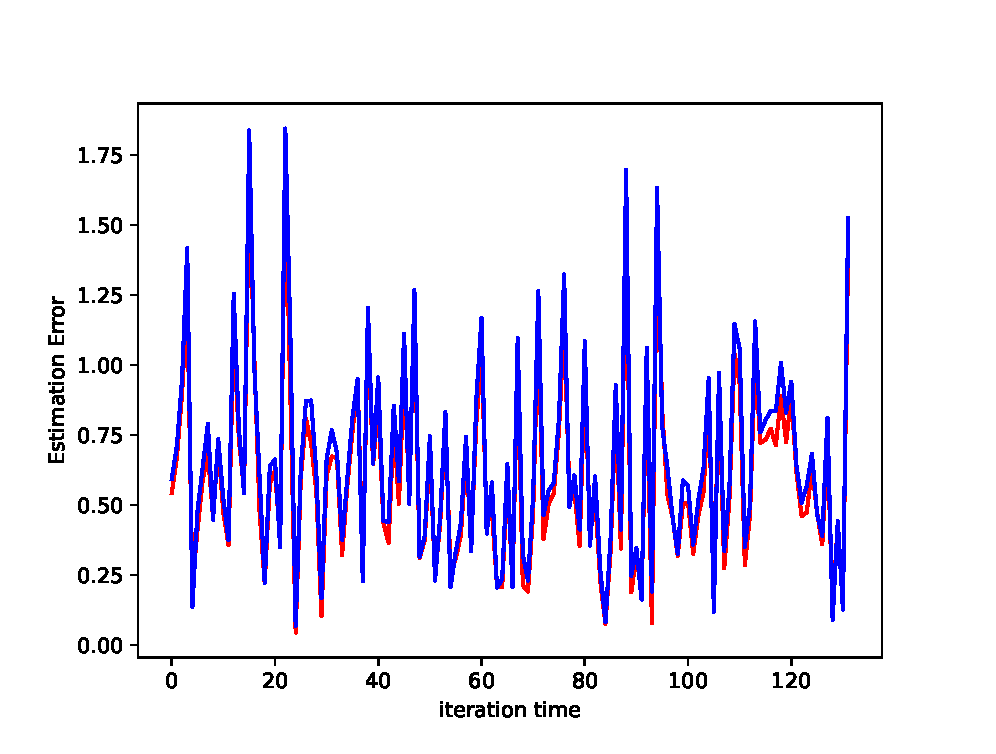
\includegraphics[width=0.5\textwidth]{./kalman_0.01.eps}
	\caption{Kalman Filter Tuning with $q_i=0.01$}
	\label{fig:kalman_tune.1}
\end{figure}
\begin{figure}[ht] 
	\centering
	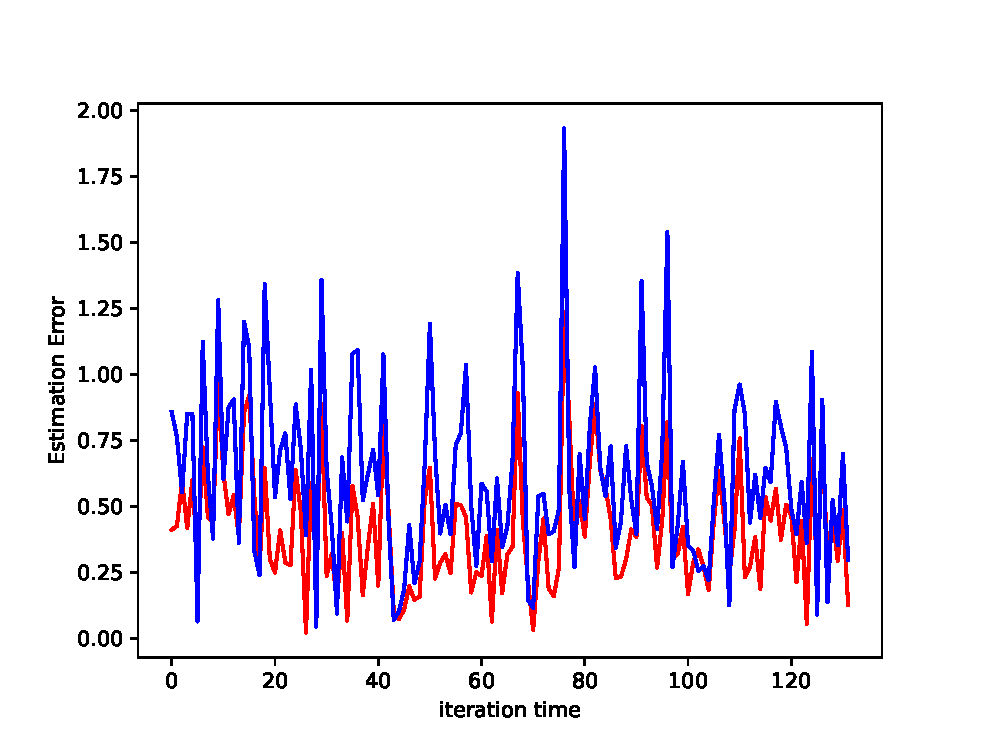
\includegraphics[width=0.5\textwidth]{./kalman_0.1.eps}
	\caption{Kalman Filter Tuning with $q_i=0.1$}
	\label{fig:kalman_tune.2}
\end{figure}
\begin{figure}[ht] 
	\centering
	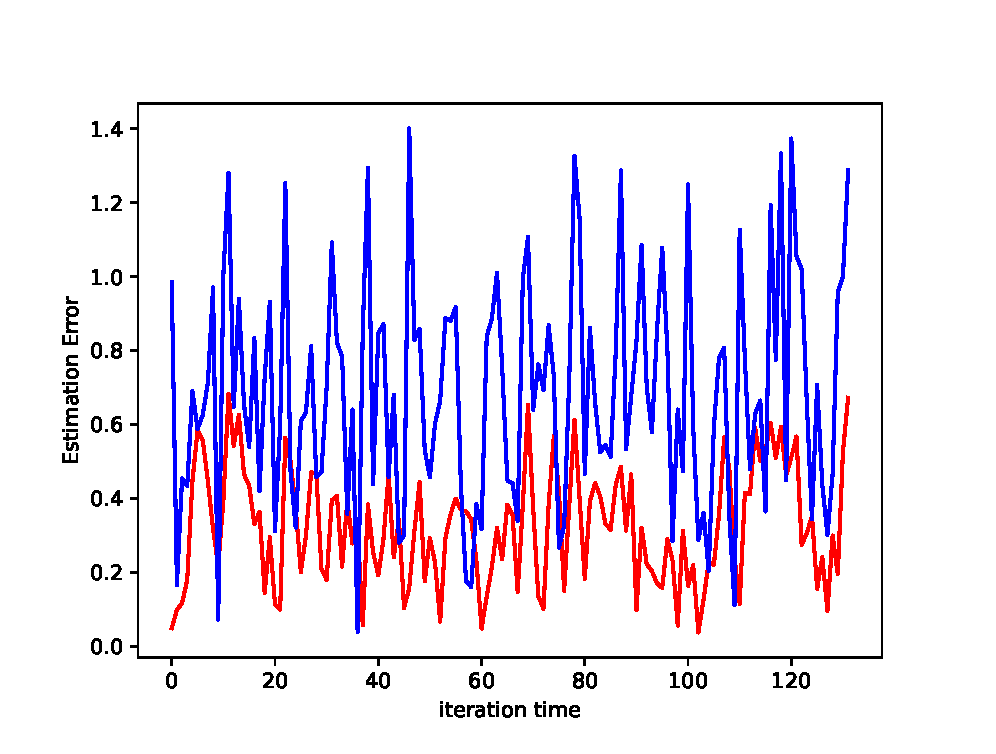
\includegraphics[width=0.5\textwidth]{./kalman_1.eps}
	\caption{Kalman Filter Tuning with $q_i=1$}
	\label{fig:kalman_tune.3}
\end{figure}
\begin{figure}[ht] 
	\centering
	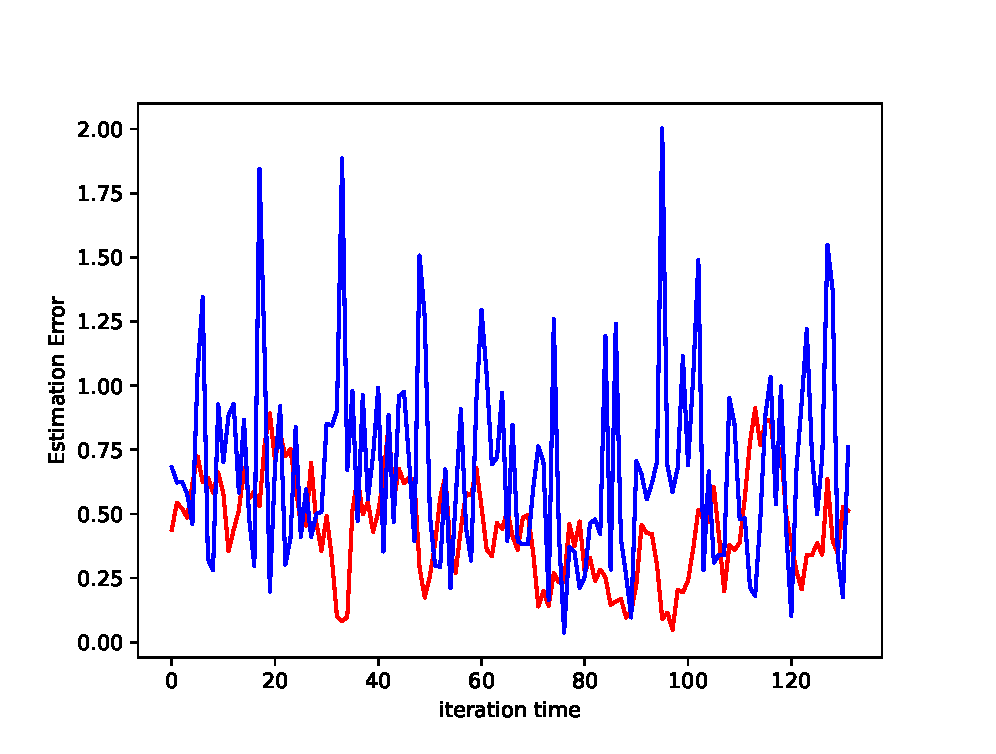
\includegraphics[width=0.5\textwidth]{./kalman_10.eps}
	\caption{Kalman Filter Tuning with $q_i=10$}
	\label{fig:kalman_tune.4}
\end{figure}


The data result for tuning are shown in table \ref{tab:kalman_tune}.

\begin{table}[]
\centering
\begin{tabular}{|c|c|c|}
\hline
$q_i$ & Error Mean & Error Variance \\ \hline
0.01  & 0.9350     & 0.0183         \\ \hline
0.1   & 0.7965     & 0.4441         \\ \hline
1     & 0.6320     & 0.6385         \\ \hline
10    & 0.9631     & 0.8548         \\ \hline
\end{tabular}
\caption{Data result for Kalman Filter Tuning}
\label{tab:kalman_tune}
\end{table}

\subsection{Particle Filter}
There's basically two parameters to tune in the particle filter: the number of points to sample and the covariance of the sampling. Here we use the same control covariance with the Kalman Filter, which is $0.1$, and test sample number of $10$, $50$, $100$ respectively. The results are shown in figure \ref{fig:particle_10}, \ref{fig:particle_50}, and \ref{fig:particle_100}. We can see that the estimation error(red line) is getting stabler when the sample number increases. According to our test, 100 samples is enough for the filter to converge. The mean and variance of the error are shown in table \ref{tab:particle_tune}, we can see that both the mean and the variance of the estimation error is decreasing, which indicates a better result.

\begin{figure}[ht] 
	\centering
	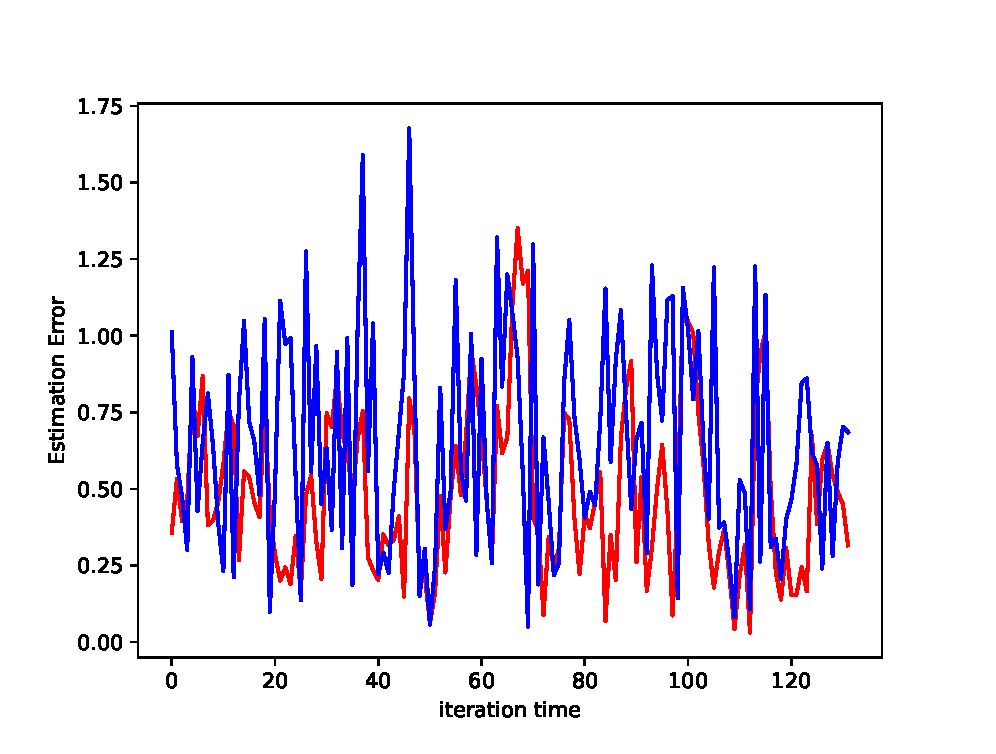
\includegraphics[width=0.5\textwidth]{./particle_10.eps}
	\caption{Particle filter with sample number 10}
	\label{fig:particle_10}
\end{figure}

\begin{figure}[ht] 
	\centering
	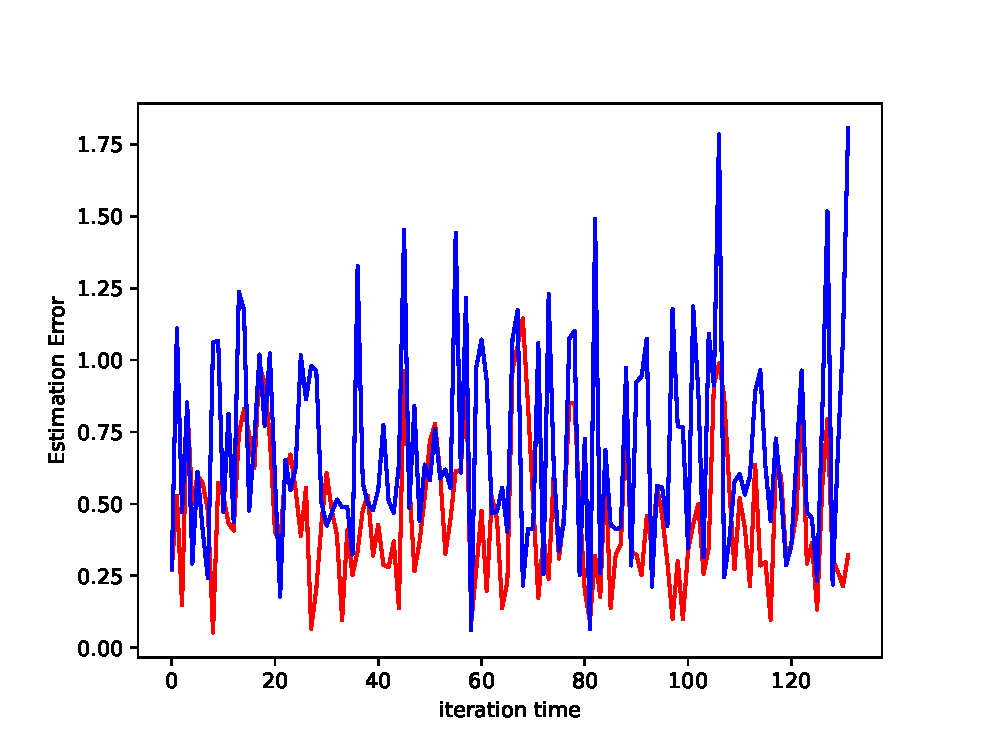
\includegraphics[width=0.5\textwidth]{./particle_50.eps}
	\caption{Particle filter with sample number 50}
	\label{fig:particle_50}
\end{figure}
\begin{figure}[ht] 
	\centering
	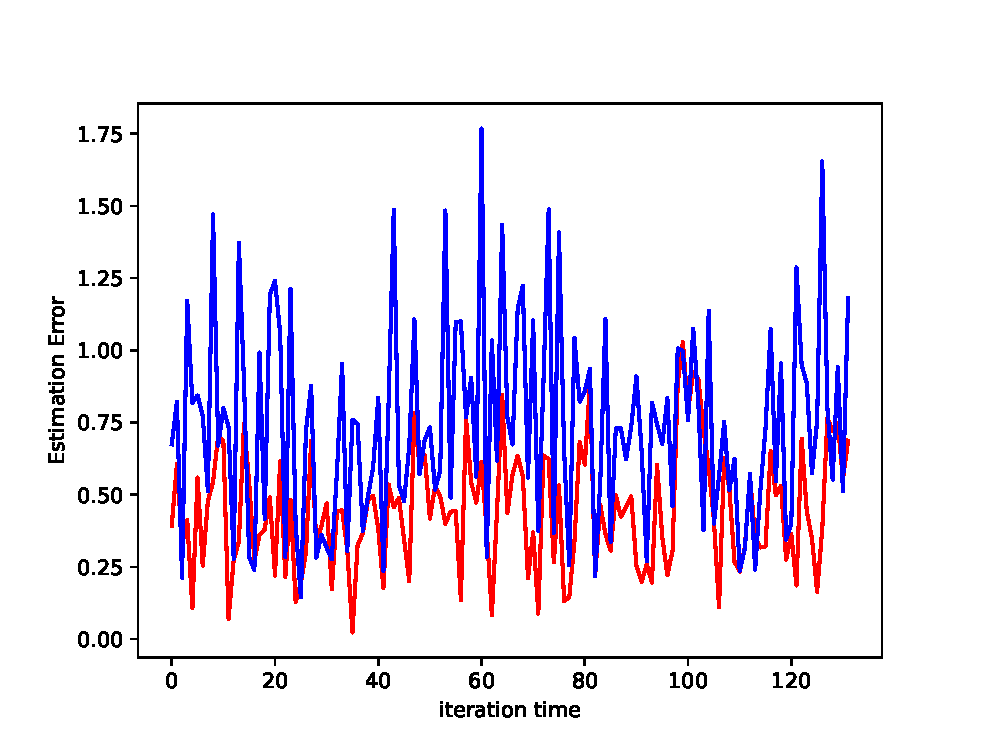
\includegraphics[width=0.5\textwidth]{./particle_100.eps}
	\caption{Particle filter with sample number 100}
	\label{fig:particle_100}
\end{figure}

\begin{table}[]
\centering
\begin{tabular}{|c|c|c|}
\hline
sample number & Error Mean & Error Variance \\ \hline
10  & 1.1041     & 4.4874         \\ \hline
50   & 0.8320     & 0.3920         \\ \hline
100     & 0.6957     & 0.1278         \\ \hline
\end{tabular}
\caption{Data result for Kalman Filter Tuning}
\label{tab:particle_tune}
\end{table}

\subsection{Kalman Filter V.S. Particle Filter}
A demonstration outcome of the program is shown in figure \ref{fig:demo_kalman} and \ref{fig:demo_particle}, where the blue line indicates the estimated trajectory and the redline is the actual trajectory of the robot. We can see that both the filters performs pretty well given that the sensor input is really noisy(error with one step). From table \ref{tab:kalman_tune} and \ref{tab:particle_tune} we can see that Kalman Filter generally performs better than the particle filter with a lower average estimation error. This is consistent to the theoretical background that the kalman filter is optimal with linear dynamics and gaussian error. What's more, kalman filter is much more efficient than particle filters which need to sample a lot of times in order to make the result converge. The efficiency is important when the algorithm is running on some embedded devices.

However, particle filter is better in error variance, which means that it performs more stable than the kalman filter when there's no disturbance such as direction change. This fact can be reflected from the demonstration. We can see that the particle filter actually performs better at the beginning.
\begin{figure}[ht]
	\centering
	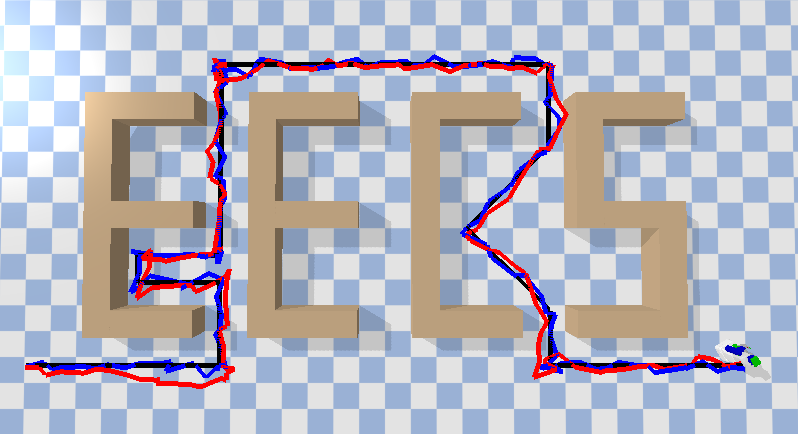
\includegraphics[width=0.5\textwidth]{./demo_kalman.png}
	\caption{Demonstration Path of the Kalman Filter}
	\label{fig:demo_kalman}
\end{figure}
\begin{figure}[ht] 
	\centering
	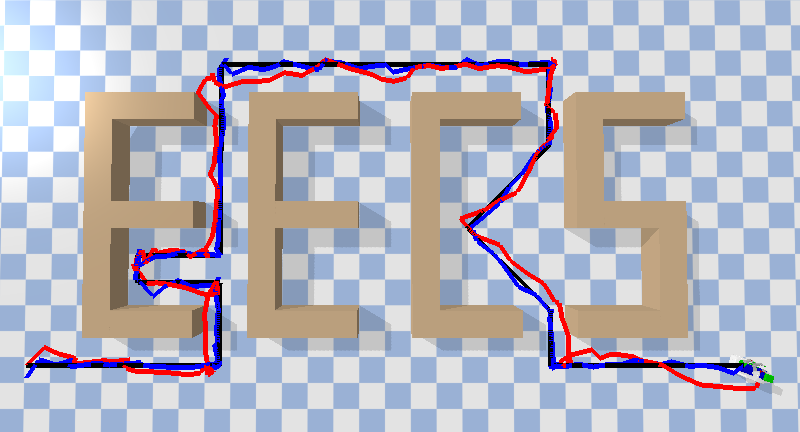
\includegraphics[width=0.5\textwidth]{./demo_particle.png}
	\caption{Demonstration Path of the Particle Filter}
	\label{fig:demo_particle}
\end{figure}


\section{Conclusion}
In this project, the performances of Kalman filter and particle filter are analyzed and compared in different scenarios.

For the Kalman filter, we can see that when the tuned ratio of sensor noise to control noise $q_i / r_i$ is closer to the actual ratio of sensor noise to control noise, the estimation performs better.

For the Particle filter, we can see that as the number of particles grow up, the estimation performs better. However, after a certain threshold is reached, the increase of number of particles don't make much difference but costs lots of computing power.

Although Kalman filter is generally much better in this case, particle filter shows more accuracy than kalman filter when there's no intense direction change, which is a case where the Kalman filter fails to produce a good estimate.

Afterall, Kalman filter performs well in terms of accuracy and efficiency in the case of linear dynamics and gaussian error, while particle is suitable for more scenarios but may be costly if the number of particles is enormous.



\begin{thebibliography}{99}

\bibitem{kf}Dmitry Berenson. "Bayes Filter and Kalman Filters." Introduction to Algorithmic Robotics. 2021, University of Michigan, Ann Arbor. Lecture.

\bibitem{particle}Dmitry Berenson. "UKF and Particle Filters." Introduction to Algorithmic Robotics. 2021, University of Michigan, Ann Arbor. Lecture.

% % \bibitem[\protect\citeauthoryear{Author}{2021}]{Author2010}
% % Dmitry Berenson. "Bayes Filter and Kalman Filters." Introduction to Algorithmic Robotics. 2021, University of Michigan, Ann Arbor. Lecture.

\end{thebibliography}

% \appendix

% \section*{Appendix: Velocity measurements}


\end{document}
